%==============================================================================
%  presentation.tex -- Soutenance d'avancement de stage (IMFT)
%  Bulle de gaz en turbulence homogene isotrope (HIT) -- DNS Basilisk
%
%  COMPILATION : pdfLaTeX (passer 2 fois pour la table des matieres / numeros).
%  Sur Overleaf : Menu > Compiler = pdfLaTeX. Aucun package exotique requis.
%==============================================================================
\documentclass[11pt,aspectratio=169]{beamer}

\usepackage[utf8]{inputenc}
\usepackage[T1]{fontenc}
\usepackage[french]{babel}
% Evite les espaces automatiques avant : ; ! ? (genants dans le code/URL)
\frenchsetup{AutoSpacePunctuation=false}
\usepackage{lmodern}
\usepackage{amsmath,amssymb,bm}
\usepackage{graphicx}
\usepackage{booktabs}
\usepackage{xcolor}
\usepackage{colortbl}   % \rowcolor dans les tableaux
\usepackage{tikz}

%--- Theme & couleurs (bleu IMFT) --------------------------------------------
\usetheme{Madrid}
\definecolor{imftblue}{RGB}{31,73,125}
\definecolor{imftlight}{RGB}{79,129,189}
\definecolor{warnred}{RGB}{170,30,30}
\definecolor{okgreen}{RGB}{34,120,60}
\usecolortheme[named=imftblue]{structure}
\setbeamercolor{palette primary}{bg=imftblue,fg=white}
\setbeamercolor{palette secondary}{bg=imftlight,fg=white}
\setbeamercolor{palette tertiary}{bg=imftblue,fg=white}
\setbeamercolor{title}{fg=imftblue}
\setbeamercolor{frametitle}{fg=imftblue}
\setbeamertemplate{navigation symbols}{}
\setbeamertemplate{caption}[numbered]
\setbeamerfont{frametitle}{series=\bfseries}
\setbeamertemplate{itemize item}{\color{imftlight}\textbullet}
\setbeamertemplate{itemize subitem}{\color{imftlight}--}

\graphicspath{{images/}}

%--- Macro : bandeau "code obsolete" -----------------------------------------
\newcommand{\oldcode}{%
  \begin{tikzpicture}[remember picture,overlay]
    \node[anchor=north east, xshift=-2mm, yshift=-1mm, fill=warnred,
          text=white, font=\scriptsize\bfseries, rounded corners=1pt,
          inner sep=2pt] at (current page.north east)
          {Resultats issus de l'ANCIEN code (obsoletes)};
  \end{tikzpicture}}

%--- Page de titre ------------------------------------------------------------
\title[Bulle en turbulence -- DNS Basilisk]{%
  Dynamique d'une bulle en turbulence homogene isotrope}
\subtitle{Simulation numerique directe (DNS) sous Basilisk --- Point d'avancement}
\author[C. Bonjean Fraser]{Carl Bonjean Fraser}
\institute[IMFT / ENSEEIHT]{%
  ENSEEIHT --- Toulouse INP \quad\textbar\quad Institut de Mecanique des Fluides de Toulouse\\[2pt]
  \footnotesize Tuteurs : D.~Legendre \& R.~Zamansky}
\date{Annee 2025--2026 \quad\textbar\quad Point d'etape semaine 5}

\titlegraphic{%
  
\includegraphics[height=1.0cm]{logo_enseeiht.png}\hspace{1.2cm}%
  
\includegraphics[height=1.0cm]{logo_imft.png}}

%==============================================================================
\begin{document}

{\setbeamertemplate{footline}{}
\begin{frame}[plain]
  \titlepage
\end{frame}}

%------------------------------------------------------------------------------
\begin{frame}{Sommaire}
  \tableofcontents
\end{frame}

%==============================================================================
\section{Contexte et objectif}
%==============================================================================
\begin{frame}{Question scientifique}
  \begin{columns}[T]
    \begin{column}{0.58\textwidth}
      \textbf{Objectif central du stage}
      \begin{quote}
        \color{imftblue}\itshape
        Une turbulence ambiante \emph{accelere}-t-elle ou \emph{ralentit}-elle
        la remontee d'une bulle de gaz ?
      \end{quote}
      \vspace{0.3em}
      \textbf{Configuration cible}
      \begin{itemize}
        \item Bulle unique, nombre de Bond $Bo = 1$ (regime deformable).
        \item Liquide en turbulence homogene isotrope (THI / HIT).
        \item Domaine 3D cubique \textbf{triplement periodique}.
        \item Fort rapport de densite $\rho_\ell/\rho_g = 850$.
      \end{itemize}
      \vspace{0.3em}
      \textbf{Finalite}
      \begin{itemize}
        \item Quantifier vitesse d'ascension, deformation, trainee.
        \item Brique vers l'etude d'un \emph{essaim} de bulles.
      \end{itemize}
    \end{column}
    \begin{column}{0.42\textwidth}
      \centering
      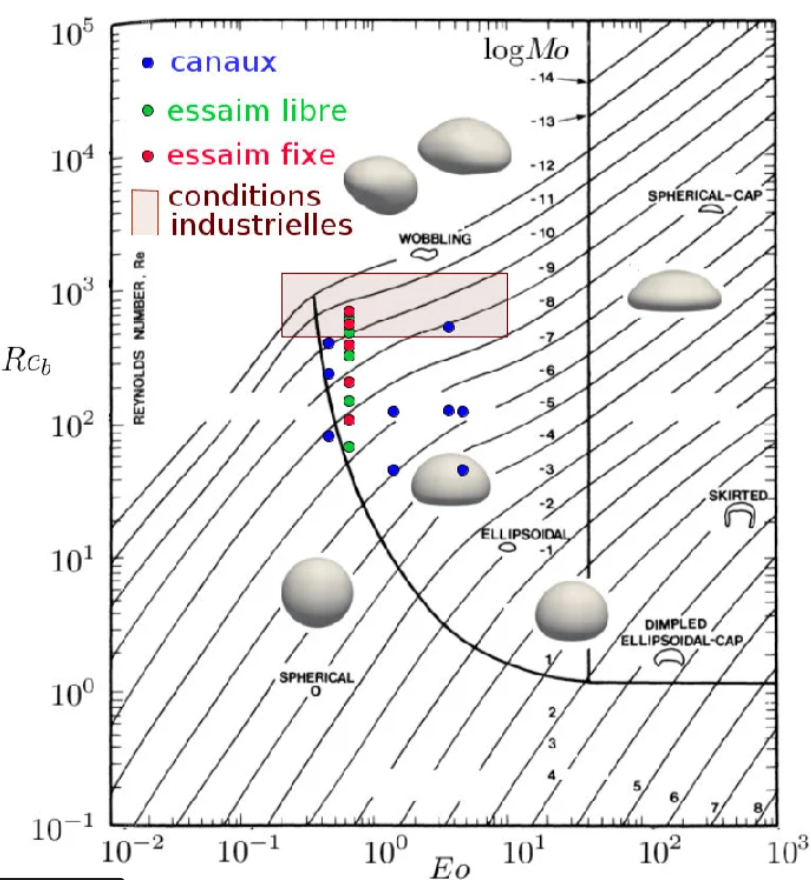
\includegraphics[width=\textwidth]{diagramme_grace.png}\\
      {\scriptsize Diagramme de Grace : nos conditions visees (encadre)
      placent la bulle en regime ellipsoidal / wobbling.}
    \end{column}
  \end{columns}
\end{frame}

\begin{frame}{Nombres adimensionnels de controle}
  \begin{columns}[T]
    \begin{column}{0.5\textwidth}
      \[ Re = \frac{\rho_\ell V D}{\mu_\ell} \qquad
         Bo = \frac{\Delta\rho\, g\, D^2}{\sigma} \]
      \[ Mo = \frac{g\,\mu_\ell^4\,\Delta\rho}{\rho_\ell^2\,\sigma^3} \]
      \begin{itemize}
        \item $Bo=1$ : flottabilite $\sim$ tension de surface.
        \item Couple $(Re,Bo)$ $\Rightarrow$ regime sur le diagramme de Grace.
        \item Cote turbulence : $We_t = \dfrac{2\rho_\ell(\varepsilon D)^{2/3}D}{\sigma}$
              pilote la fragmentation.
      \end{itemize}
    \end{column}
    \begin{column}{0.5\textwidth}
      \footnotesize
      \textbf{Unites du code} ($\rho_1=1,\ g=1,\ L_0=120$) :
      \begin{itemize}
        \item Rayon bulle $R_0 = 4{,}24$ (longueur de reference).
        \item $Bo = \rho_1 g (2R_0)^2/\sigma = 1$ impose la \emph{tension de
              surface dynamiquement} (jamais codee en dur).
        \item Gravite reduite $G_z = -1$ : la phase legere (gaz) remonte en $+z$.
      \end{itemize}
      \vspace{0.4em}
      \begin{block}{Convention bulle = gaz}
        La bulle est la phase $f<0{,}5$ (VOF). $G_z<0 \Rightarrow$ remontee
        de la phase legere.
      \end{block}
    \end{column}
  \end{columns}
\end{frame}

\begin{frame}{Methode numerique : pourquoi de l'ILES sous Basilisk}
  \begin{columns}[T]
    \begin{column}{0.62\textwidth}
      \begin{itemize}
        \item \textbf{DNS pure} : toutes les echelles jusqu'a Kolmogorov $\eta$.
              Exact mais $N_{\text{mailles}}\sim Re^{9/4}$ $\rightarrow$ milliards
              de cellules. \textcolor{warnred}{Ecarte.}
        \item \textbf{RANS} : moyennes temporelles, viscosite turbulente.
              Tue la dynamique d'interface. \textcolor{warnred}{Ecarte.}
        \item \textbf{ILES} : grandes echelles resolues, dissipation sous-maille
              \emph{implicite} via le schema. \textcolor{okgreen}{Retenu}, natif
              dans Basilisk via le maillage adaptatif (\texttt{adapt\_wavelet}).
      \end{itemize}
    \end{column}
    \begin{column}{0.38\textwidth}
      \footnotesize
      \begin{block}{Briques Basilisk}
        \begin{itemize}
          \item \texttt{octree} : maillage adaptatif 3D (AMR).
          \item \texttt{two-phase} + \texttt{tension} : interface VOF.
          \item \texttt{conserving} : advection conservant la qdm (haut $\rho_\ell/\rho_g$).
          \item \texttt{reduced} : gravite well-balanced (domaine periodique).
        \end{itemize}
      \end{block}
      Calcul sur supercalculateur (\textbf{Kairos}, IMFT ; acces \textbf{CALMIP/Olympe}).
    \end{column}
  \end{columns}
\end{frame}

%==============================================================================
\section{Journal de bord semaine par semaine}
%==============================================================================
\begin{frame}{Vue d'ensemble du planning}
  \footnotesize
  \begin{tabular}{@{}p{1.3cm}p{7.0cm}p{4.2cm}@{}}
    \toprule
    \textbf{Semaine} & \textbf{Travail realise} & \textbf{Livrable / probleme} \\
    \midrule
    S1 & Installation (WSL, \texttt{qcc}), prise en main 2D, biblio
       & Cas-tests 2D valides \\
    S2 & Passage 3D, forcage turbulent, run exploratoire lvl 8
       & \textcolor{warnred}{Inversion des phases} \\
    S3 & Protocole \emph{precurseur $\to$ injection}, etude de convergence 7/8/9
       & Premiere caracterisation THI \\
    S4 & \textcolor{warnred}{Refonte du code} (adaptation defaillante), optimisation HPC
       & Code precis actuel \\
    S5 & Precurseur lvl 9 sur Kairos $\to$ cloture partie 1
       & \emph{(en cours)} \\
    \rowcolor{imftlight!15}
    Suite & Etude : intensite turbulente $\to$ vitesse d'ascension
       & Objectif principal \\
    \bottomrule
  \end{tabular}
  \vspace{0.6em}
  \begin{center}
    \scriptsize\itshape
    Fil rouge : passer d'un code 2D pedagogique a un solveur DNS 3D
    quantitatif et reproductible.
  \end{center}
\end{frame}

\begin{frame}{Semaine 1 --- Prise en main \& cas-tests 2D}
  \begin{columns}[T]
    \begin{column}{0.5\textwidth}
      \begin{itemize}
        \item Environnement UNIX (WSL/Ubuntu), compilateur \texttt{qcc},
              outils de rendu Basilisk.
        \item Apprentissage du C et des routines Basilisk (\emph{two-phase flows}).
        \item \textbf{Bulle isolee 2D} ($Ga=100$, $Bo=10$) : trajectoire en
              \emph{zigzag}, lachers tourbillonnaires (allee de von K\'arm\'an).
        \item \textbf{Turbulence 2D decroissante} (formulation $\omega$--$\psi$) :
              cascade \emph{inverse}, fusion des structures.
        \item Biblio : revue D.~Legendre sur la dynamique des bulles.
      \end{itemize}
    \end{column}
    \begin{column}{0.5\textwidth}
      \centering
      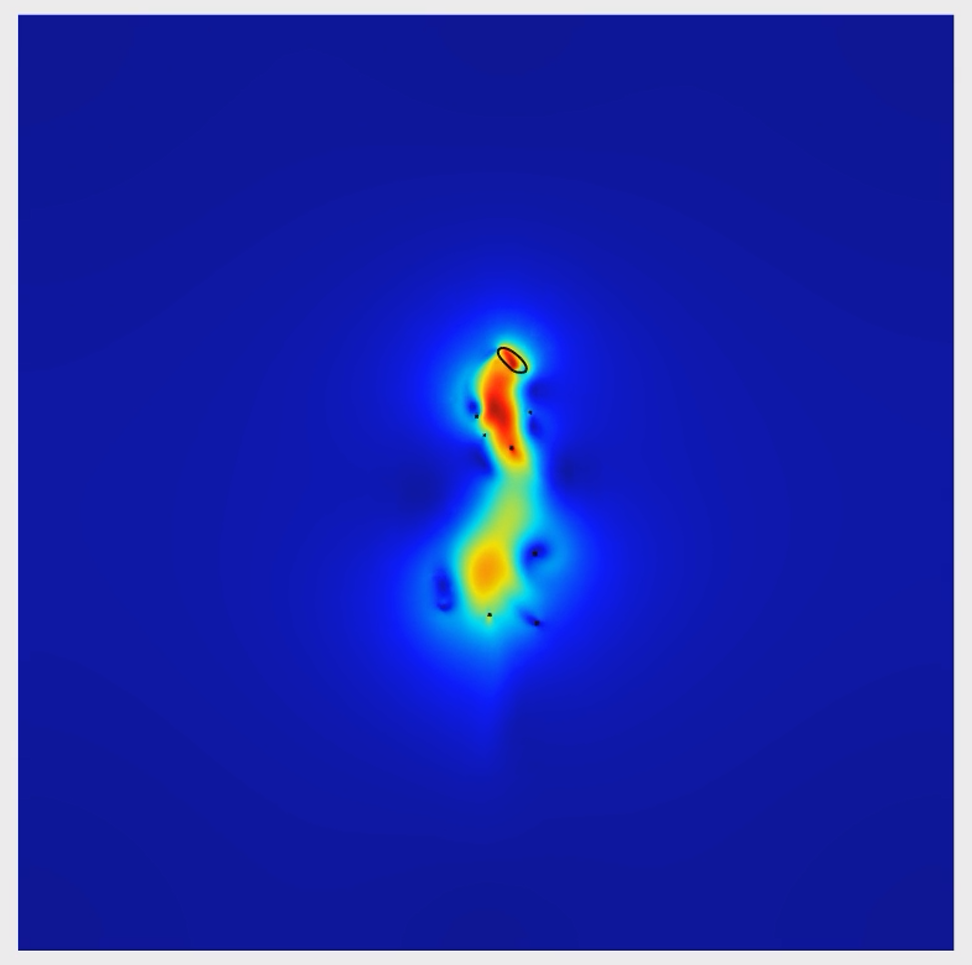
\includegraphics[height=2.7cm]{bulle2d_zigzag.png}\hfill
      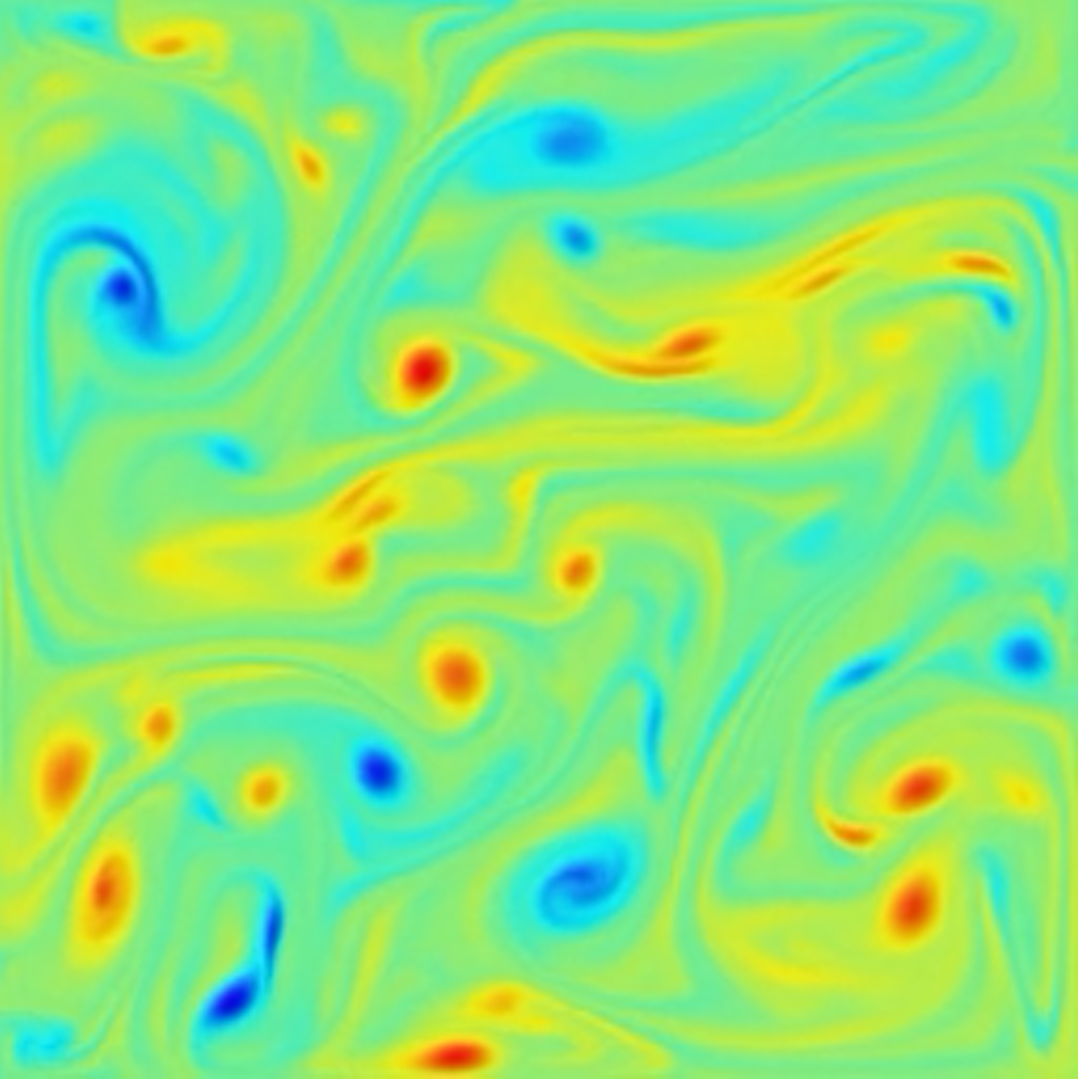
\includegraphics[height=2.7cm]{turbulence2d.png}\\[2pt]
      {\scriptsize Gauche : sillage \& jet vertical d'une bulle 2D en zigzag.
       Droite : champ de vorticite d'une THI 2D decroissante.}
    \end{column}
  \end{columns}
\end{frame}

\begin{frame}{Semaine 2 --- Passage en 3D et premier ecueil}
  \begin{columns}[T]
    \begin{column}{0.56\textwidth}
      \begin{itemize}
        \item Ecriture d'un solveur 3D triplement periodique.
        \item \textbf{Forcage lineaire} de la THI : terme source
              $\propto (u - \bar u)$ pour compenser la dissipation visqueuse.
        \item Run exploratoire lvl 8 ($\sim$8 h de calcul) : dynamique de calotte.
        \item Ouverture des acces \textbf{CALMIP / Olympe}.
      \end{itemize}
      \vspace{0.3em}
      \begin{alertblock}{Probleme rencontre}
        Au post-traitement : \textbf{phases inversees} (gaz $\leftrightarrow$
        liquide). $\Rightarrow$ simulations a refaire en S3 avec la bonne
        configuration physique.
      \end{alertblock}
    \end{column}
    \begin{column}{0.44\textwidth}
      \centering
      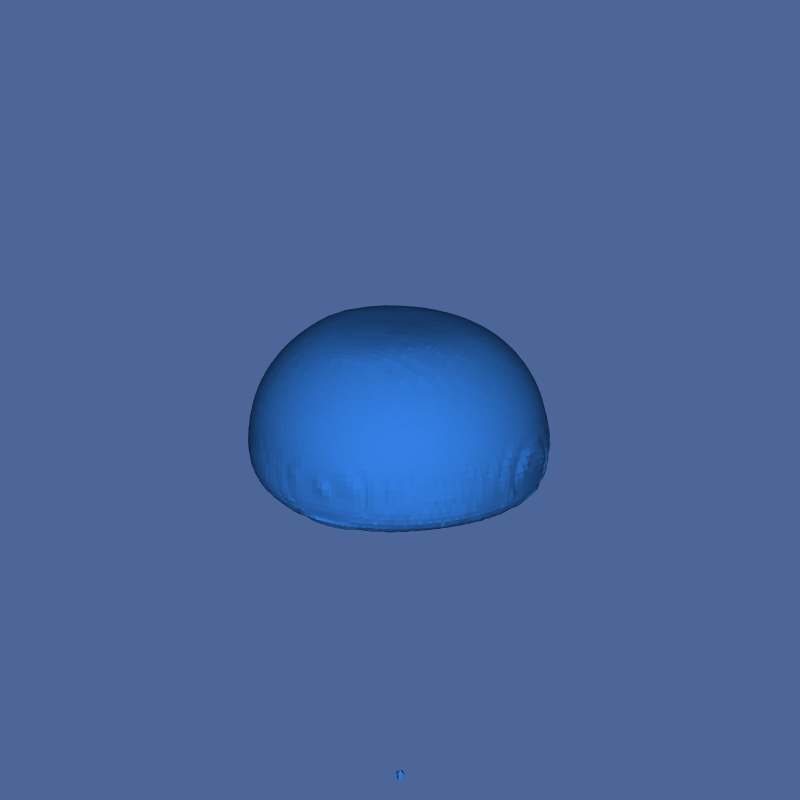
\includegraphics[height=3.4cm]{bulle3d_calotte.png}\\[2pt]
      {\scriptsize Bulle 3D en calotte spherique (rendu d'interface VOF,
       maillage grossier lvl 7).}
    \end{column}
  \end{columns}
\end{frame}

\begin{frame}{Semaine 3 --- Le protocole \og precurseur \fg{}}
  \begin{columns}[T]
    \begin{column}{0.55\textwidth}
      \textbf{Idee :} ne pas injecter la bulle dans un fluide au repos, mais
      dans une \emph{turbulence deja developpee et statistiquement stationnaire}.
      \vspace{0.4em}
      \begin{enumerate}
        \item \textbf{Phase 1 -- Precurseur} (\texttt{INJECT=0}) :
              champ ABC monophasique $\to$ THI forcee, sans interface.
              On laisse s'etablir l'etat stationnaire, puis on \emph{dump} le
              champ final (\texttt{end}).
        \item \textbf{Phase 2 -- Bulle} (\texttt{INJECT=1}) :
              on \emph{restaure} ce champ, on raffine autour de la sphere,
              on injecte la bulle (VOF) et on la laisse remonter.
      \end{enumerate}
    \end{column}
    \begin{column}{0.45\textwidth}
      \begin{block}{Pourquoi cette etape ?}
        \footnotesize
        \begin{itemize}
          \item Injecter dans une turbulence \emph{mure} (spectre developpe), pas
                un transitoire artificiel.
          \item Un seul precurseur (cher) re-servi pour plusieurs runs bulle.
          \item Separe proprement \emph{etablissement de la THI} et
                \emph{interaction bulle--turbulence}.
        \end{itemize}
      \end{block}
      \footnotesize
      \textit{Inspiration : sandbox W.~Mostert, \texttt{turbulent\_bubble.c}
      (cf. references).}
    \end{column}
  \end{columns}
\end{frame}

%==============================================================================
\section{Premiere caracterisation de la turbulence (ancien code)}
%==============================================================================
\begin{frame}{Premiere caracterisation de la THI --- precurseur}
  \oldcode
  \begin{columns}[T]
    \begin{column}{0.62\textwidth}
      \centering
      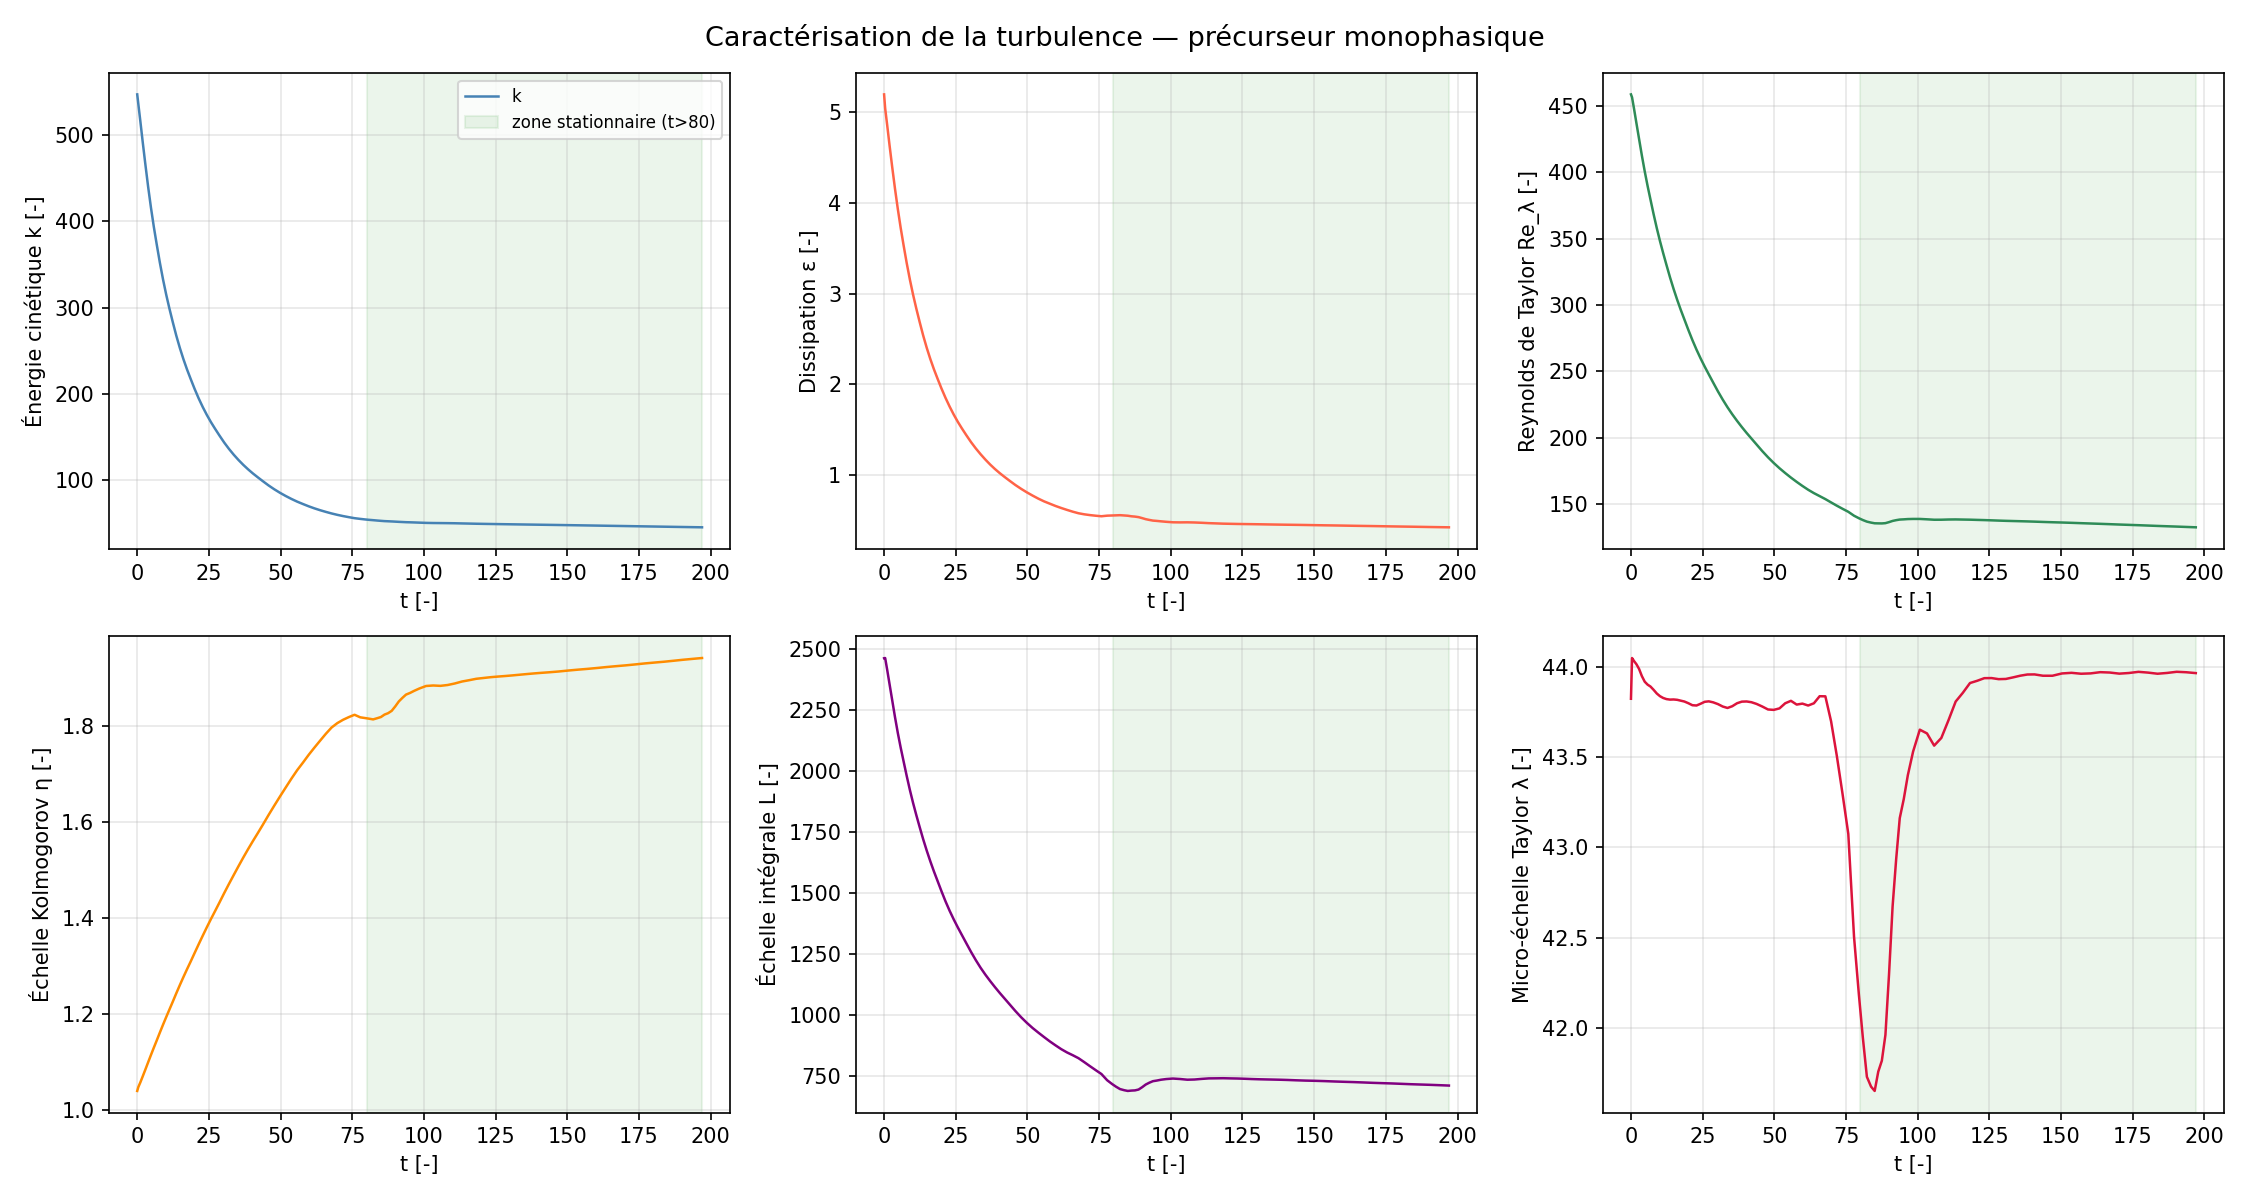
\includegraphics[width=\textwidth]{turbulence_carac_precurseur.png}
    \end{column}
    \begin{column}{0.38\textwidth}
      \footnotesize
      Suivi temporel des grandeurs THI du precurseur (lvl 7/8) :
      \begin{itemize}
        \item $k$ : energie cinetique turbulente,
        \item $\varepsilon$ : dissipation,
        \item $Re_\lambda$ : Reynolds de Taylor,
        \item $\eta$, $L$, $\lambda$ : echelles de Kolmogorov, integrale, Taylor.
      \end{itemize}
      \vspace{0.3em}
      \begin{block}{Lecture}
        Etablissement d'un \textbf{plateau stationnaire} (zone verte, $t>80$) :
        $Re_\lambda \approx 137$, $\varepsilon \approx 0{,}47$. C'est l'etat
        \emph{a partir duquel} on injecte la bulle.
      \end{block}
    \end{column}
  \end{columns}
\end{frame}

\begin{frame}{Spectre d'energie --- cascade turbulente}
  \oldcode
  \begin{columns}[T]
    \begin{column}{0.6\textwidth}
      \centering
      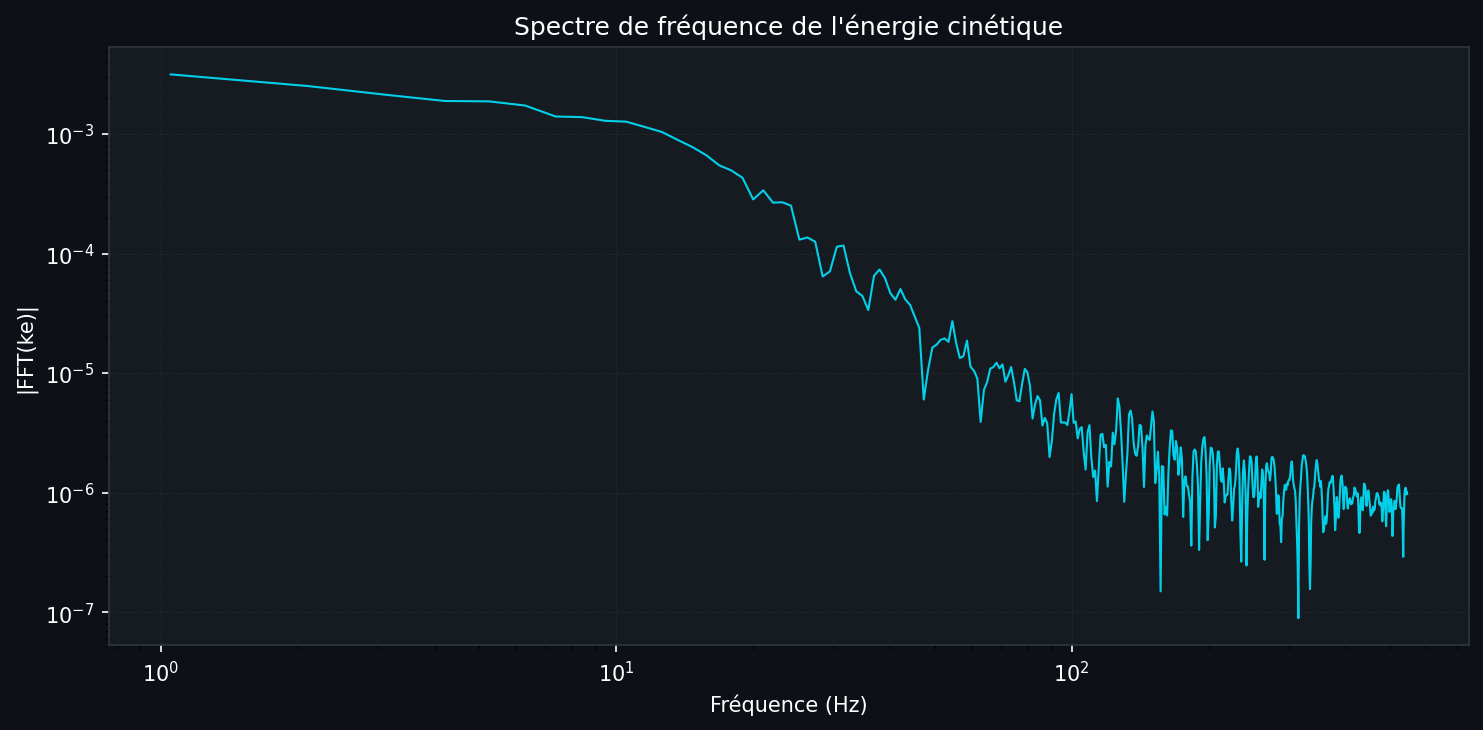
\includegraphics[width=\textwidth]{spectre_ke.png}
    \end{column}
    \begin{column}{0.4\textwidth}
      \footnotesize
      \begin{itemize}
        \item Spectre frequentiel de l'energie cinetique (FFT du signal $k(t)$).
        \item Plateau aux \textbf{grandes echelles} (forcage), puis decroissance
              regularie vers les \textbf{petites echelles} dissipatives.
        \item Confirme qualitativement une cascade d'energie bien etablie
              dans le precurseur.
      \end{itemize}
      \vspace{0.4em}
      \textit{La caracterisation propre (spectre spatial $E(k)$, pente $-5/3$)
      sera refaite sur le nouveau precurseur lvl 9.}
    \end{column}
  \end{columns}
\end{frame}

\begin{frame}{Etude de convergence 7/8/9 --- et le probleme cache}
  \oldcode
  \footnotesize
  \begin{columns}[T]
    \begin{column}{0.54\textwidth}
      \begin{tabular}{lccc}
        \toprule
        \textbf{Grandeur} & \textbf{lvl 7} & \textbf{lvl 8} & \textbf{lvl 9} \\
        \midrule
        $\Delta x$              & $0{,}94$ & $0{,}47$ & $0{,}23$ \\
        $k$                     & $48{,}7$ & $49{,}3$ & $36{,}5^\star$ \\
        $Re_\lambda$            & $137$    & $137$    & $102^\star$ \\
        \midrule
        Volume bulle            & $3{,}3$  & $17$     & $150$ \\
        $V/V_{th}$ [\%]         & $1$      & $5$      & $45$ \\
        Nb fragments            & $1$      & $1$      & $1$ \\
        \bottomrule
      \end{tabular}
      \vspace{0.4em}\\
      {\scriptsize $^\star$ precurseur lvl 9 non encore stationnaire.}
    \end{column}
    \begin{column}{0.46\textwidth}
      \begin{alertblock}{Anomalie}
        Perte de \textbf{50 a 99\,\%} du volume theorique
        ($V_{th}\approx 333$) \emph{des l'injection}, et qui ne se corrige pas
        en raffinant.
      \end{alertblock}
      Un raffinement a $\Delta x = 0{,}23$ ($\sim$37 mailles/diametre) devrait
      conserver le volume a mieux que 1\,\%. \\
      \textcolor{warnred}{\textbf{Quelque chose ne va pas dans le maillage.}}
    \end{column}
  \end{columns}
\end{frame}

\begin{frame}{Diagnostic : une adaptation de maillage defaillante}
  \begin{columns}[T]
    \begin{column}{0.55\textwidth}
      \begin{alertblock}{Cause racine}
        Le critere de l'\texttt{event adapt} de l'ancien code etait
        \textbf{beaucoup trop laxiste}.
      \end{alertblock}
      \begin{itemize}
        \item Le seuil d'ondelette ne declenchait jamais le raffinement
              jusqu'a \texttt{maxlevel}.
        \item Consequence : \textbf{lvl 7, 8 et 9 donnaient le \emph{meme}
              nombre de cellules}.
        \item L'\og etude de convergence\fg{} comparait donc \emph{trois fois le
              meme maillage} effectif $\Rightarrow$ resultats incoherents
              (volume, $V/V_{th}$).
        \item La bulle, mal resolue au moment du \texttt{fraction()}, perdait son
              volume instantanement.
      \end{itemize}
    \end{column}
    \begin{column}{0.45\textwidth}
      \begin{block}{Decision (fin S3 / S4)}
        \textcolor{warnred}{\textbf{Refonte complete du solveur}} pour rendre
        l'adaptation reellement pilotee par le niveau, et garantir une bulle
        bien resolue a l'injection.
      \end{block}
      \centering
      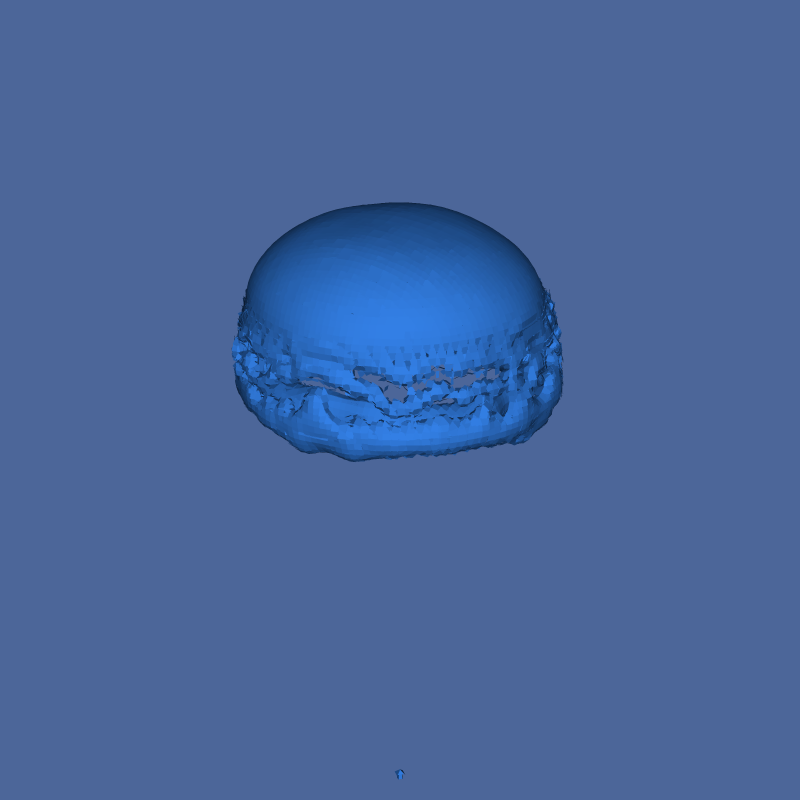
\includegraphics[height=2.6cm]{bulle3d_rupture.png}\\
      {\scriptsize Interface mal resolue : decrochage / \og rupture\fg{}
       numerique parasite.}
    \end{column}
  \end{columns}
\end{frame}

%==============================================================================
\section{Semaine 4 : refonte du code et HPC}
%==============================================================================
\begin{frame}{Semaine 4 --- Ce qui a change dans le code}
  \footnotesize
  \begin{columns}[T]
    \begin{column}{0.5\textwidth}
      \textbf{Corrections cles}
      \begin{itemize}
        \item \texttt{adapt\_wavelet} sur \textbf{l'interface ET la vitesse}
              $\{f, u_x, u_y, u_z\}$, seuils \emph{fixes} et identiques aux 3
              niveaux (on isole le seul effet de la resolution).
        \item \texttt{refine()} d'une \textbf{coquille} autour de la sphere
              \emph{avant} l'appel a \texttt{fraction()} $\to$ bulle bien
              resolue des l'injection.
        \item Bulle-mere = plus gros volume de gaz (\texttt{tag}) ; vitesse
              $u_z = \int (1-f)u_z / \int (1-f)$.
        \item Centre de masse par \textbf{moyenne circulaire} (robuste a la
              periodicite).
        \item Toutes les ecritures \texttt{.dat} protegees par
              \texttt{if(pid()==0)} (MPI propre).
      \end{itemize}
    \end{column}
    \begin{column}{0.5\textwidth}
      \begin{block}{Le critere d'adaptation, corrige}
        \ttfamily\scriptsize
        uemax = 0.02*(WIDTH/(2*pi));\\
        femax = 1e-3;\\
        adapt\_wavelet(\{f,u.x,u.y,u.z\},\\
        ~~~\{femax,uemax,uemax,uemax\},\\
        ~~~maxlevel);
      \end{block}
      \begin{block}{Nouveau diagnostic \texttt{cells.dat}}
        \scriptsize
        Compte global de cellules a chaque pas $\to$ on \emph{voit} enfin le
        maillage grossir avec le niveau, et on dimensionne les coeurs
        ($\sim$100k cellules/coeur).
      \end{block}
    \end{column}
  \end{columns}
\end{frame}

\begin{frame}{Semaine 4 --- Optimisation HPC (et canicule)}
  \begin{columns}[T]
    \begin{column}{0.58\textwidth}
      \begin{itemize}
        \item Conditions de travail extremes (canicule $\sim 40^\circ$C)
              $\rightarrow$ reorientation vers l'organisation et l'optimisation
              de l'usage du calculateur.
        \item Apprentissage du \textbf{profilage CPU en direct} (avec l'aide de
              B.~Gautam).
        \item Regle empirique de dimensionnement :
              \textbf{1 tache MPI pour 1 a 5$\times 10^4$ cellules}, ajustee selon
              l'evolution du maillage adaptatif.
        \item Run lvl 9 distribue efficacement ; passage a $maxlevel=9$ a exige
              d'\textbf{assouplir la tolerance temporelle} et d'autoriser plus
              d'iterations du solveur (instabilites de convergence).
      \end{itemize}
    \end{column}
    \begin{column}{0.42\textwidth}
      \begin{block}{Parametres numeriques}
        \footnotesize
        \begin{itemize}
          \item \texttt{TOLERANCE = 1e-4}
          \item \texttt{CFL = 0.5}
          \item $N_{\text{base}} = 2^{\,maxlevel-3}$
          \item Checkpoint glissant \texttt{dump} $\to$ \textbf{reprise auto}
                apres une limite de temps SLURM.
        \end{itemize}
      \end{block}
      \footnotesize
      Le \texttt{dump} glissant rend chaque run \emph{redemarrable} : indispensable
      pour des calculs de plusieurs dizaines d'heures.
    \end{column}
  \end{columns}
\end{frame}

%==============================================================================
\section{Le code actuel : fonctionnement et sorties}
%==============================================================================
\begin{frame}{Comment fonctionne le code actuel (pipeline 2 phases)}
  \centering
  \resizebox{0.92\textwidth}{!}{%
  \begin{tikzpicture}[
    b/.style={draw, rounded corners, fill=imftlight!15, text width=2.3cm,
              align=center, minimum height=0.95cm, inner sep=3pt, font=\scriptsize},
    a/.style={->, thick, imftblue}]
    \node[b] (pre) at (0,0)    {\textbf{Precurseur}\\\texttt{INJECT=0}};
    \node[b] (end) at (3.2,0)  {\textbf{Etat stationnaire}\\dump \texttt{end}};
    \node[b] (bub) at (6.4,0)  {\textbf{Bulle}\\\texttt{INJECT=1}};
    \node[b] (out) at (9.6,0)  {\textbf{Remontee}\\\texttt{bubble.dat}};
    \draw[a] (pre) -- (end);
    \draw[a] (end) -- node[above]{\scriptsize restart} (bub);
    \draw[a] (bub) -- (out);
  \end{tikzpicture}}

  \vspace{1.0em}

  \begin{columns}[T]
    \begin{column}{0.5\textwidth}
      \begin{block}{Lancer toute la chaine}
        {\scriptsize\ttfamily ./run\_pipeline.sh}\\[1pt]
        {\scriptsize precurseur lvl9 $\to$ bulle lvl 7/8/9}
      \end{block}
    \end{column}
    \begin{column}{0.5\textwidth}
      \begin{block}{Un cas seul}
        {\scriptsize\ttfamily ./bubble 9 60 8.0 1 0.1 1}\\[1pt]
        {\scriptsize\itshape maxlevel MAXTIME R0 FORCED amp INJECT}
      \end{block}
    \end{column}
  \end{columns}
\end{frame}

\begin{frame}{Ce que le code produit en sortie}
  \footnotesize
  \begin{tabular}{@{}p{2.6cm}p{9.5cm}@{}}
    \toprule
    \textbf{Fichier} & \textbf{Contenu} \\
    \midrule
    \texttt{stats.dat}   & \texttt{t} \quad dissipation $\varepsilon$ \quad energie $k$ \quad Reynolds (THI du liquide) \\
    \texttt{bubble.dat}  & \texttt{t volume xc yc zc ux uy uz width depth height d\_eq chi}
                           $\to$ trajectoire, vitesse d'ascension $u_z$, rapport d'aspect $\chi$ \\
    \texttt{cells.dat}   & \texttt{i t cells} : suivi du nombre de cellules (dimensionnement coeurs) \\
    \texttt{dump}        & checkpoint glissant (reprise automatique) \\
    \texttt{snapshot-*}  & instantanes pour le rendu 3D offline \\
    \texttt{end}         & champ final du precurseur (= \texttt{restart} des runs bulle) \\
    \bottomrule
  \end{tabular}
  \vspace{0.6em}
  \begin{block}{Post-traitement (\texttt{scripts/postprocess.py})}
    \footnotesize
    Produit : \texttt{rise\_velocity.png} (vitesse $u_z(t)$ par niveau),
    \texttt{convergence.png} (vitesse terminale vs \texttt{maxlevel}),
    \texttt{aspect\_ratio.png}, \texttt{turbulence.png} et un
    \texttt{convergence\_table.csv}. La convergence spatiale est acceptee quand
    l'ecart lvl8$\to$lvl9 sur $u_z$ terminal est faible (qq \%).
  \end{block}
\end{frame}

\begin{frame}{Etat actuel du calcul (semaine 5)}
  \begin{columns}[T]
    \begin{column}{0.58\textwidth}
      \begin{block}{En cours sur Kairos}
        Precurseur \textbf{monophasique lvl 9} en train de tourner.
        Objectif : atteindre l'etat statistiquement stationnaire a la resolution
        fine, ce qui n'avait jamais ete obtenu proprement auparavant.
      \end{block}
      \textbf{Des qu'il est stationnaire :}
      \begin{itemize}
        \item \textbf{Caracterisation propre de la THI} lvl 9 ($k$, $\varepsilon$,
              $Re_\lambda$, spectre $E(k)$) --- la \emph{vraie} version de la
              caracterisation montree precedemment.
        \item Il servira de \texttt{restart} commun aux runs bulle.
      \end{itemize}
    \end{column}
    \begin{column}{0.42\textwidth}
      \centering
      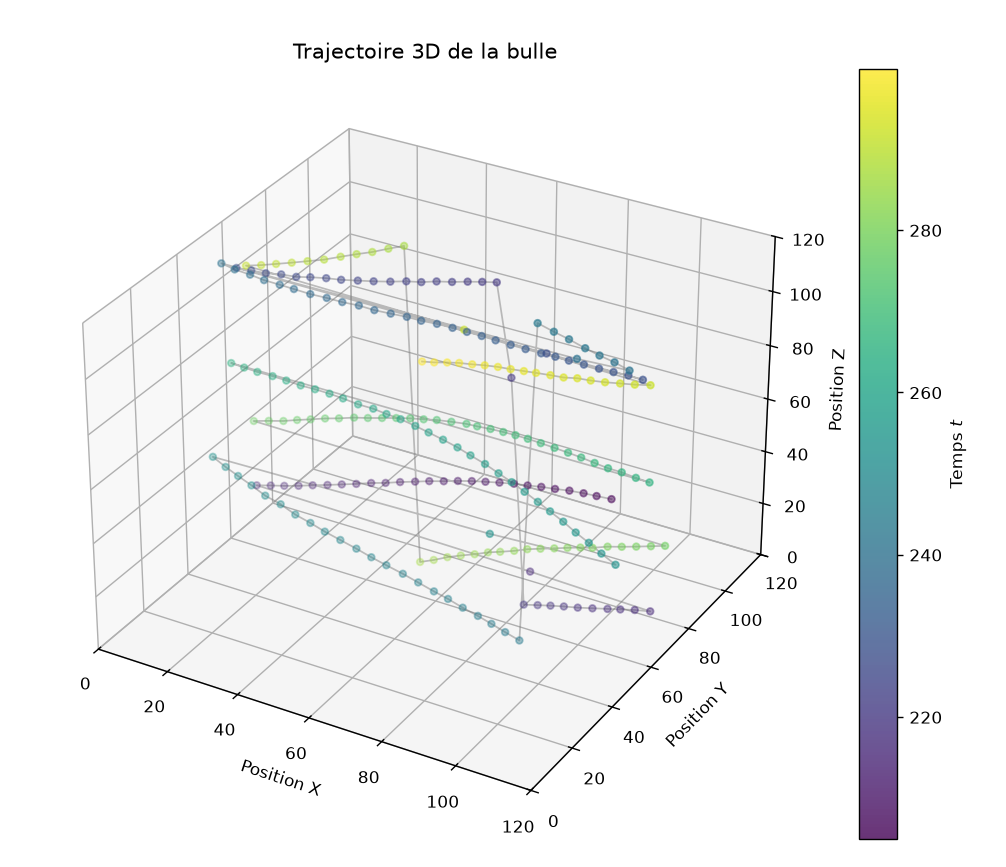
\includegraphics[width=\textwidth]{trajectoire3d.png}\\
      {\scriptsize Trajectoire 3D d'une bulle
       \textcolor{warnred}{(ancien code)} : les sauts horizontaux sont les
       traversees de frontiere periodique, corrigees par la moyenne circulaire
       du centre de masse.}
    \end{column}
  \end{columns}
\end{frame}

%==============================================================================
\section{Resultats illustratifs (a confirmer)}
%==============================================================================
\begin{frame}{Resultats presentables aujourd'hui}
  \oldcode
  \begin{columns}[c]
    \begin{column}{0.33\textwidth}
      \centering
      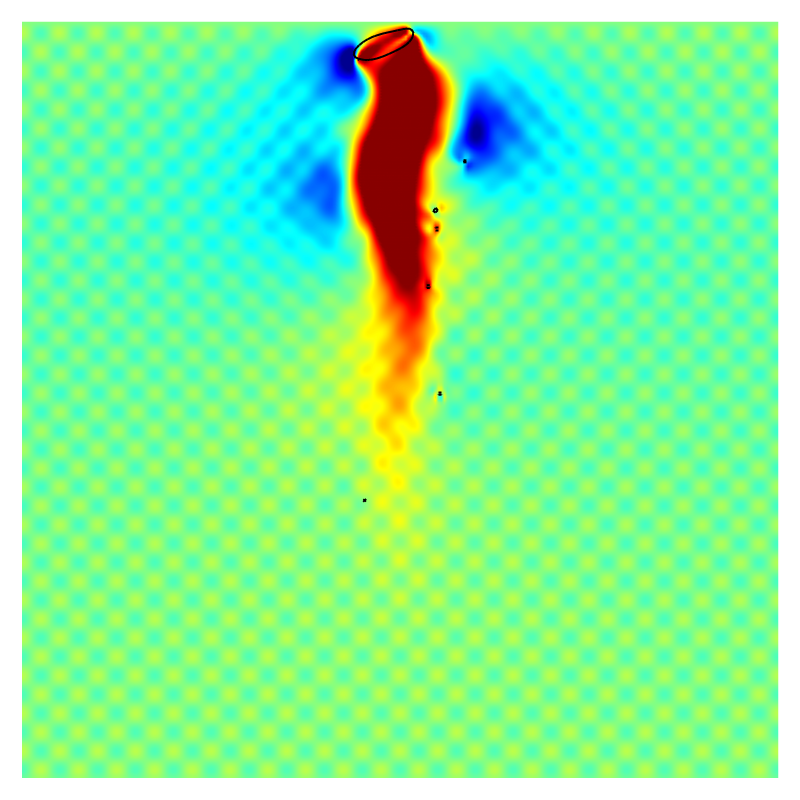
\includegraphics[width=\textwidth]{bulle2d_turbulence.png}\\
      {\scriptsize Bulle 2D dans turbulence forcee : jet ascendant + sillage.}
    \end{column}
    \begin{column}{0.33\textwidth}
      \centering
      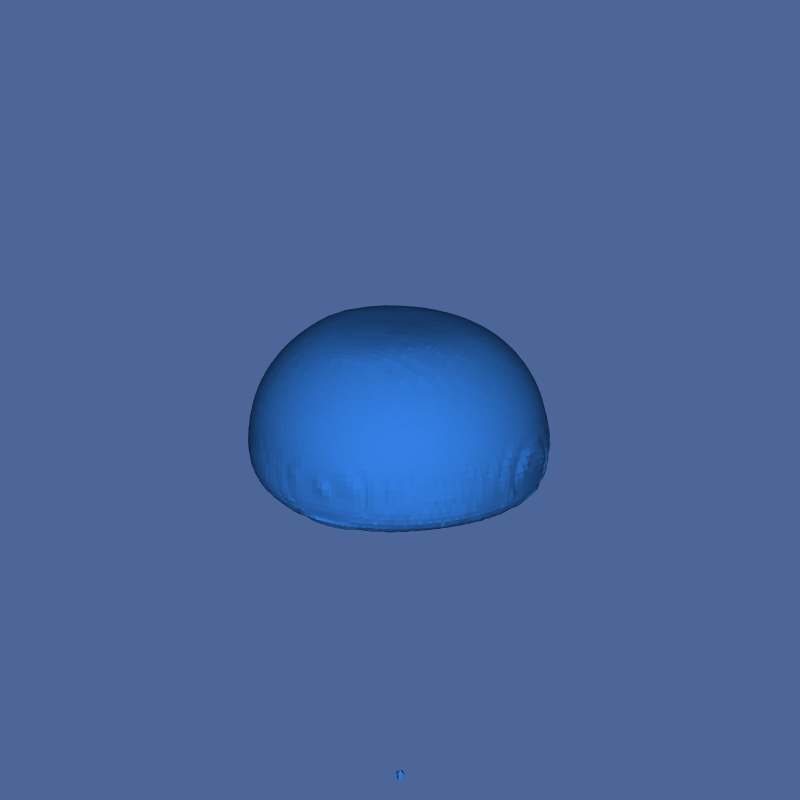
\includegraphics[width=\textwidth]{bulle3d_calotte.png}\\
      {\scriptsize Calotte 3D, interface VOF (rendu offline).}
    \end{column}
    \begin{column}{0.33\textwidth}
      \centering
      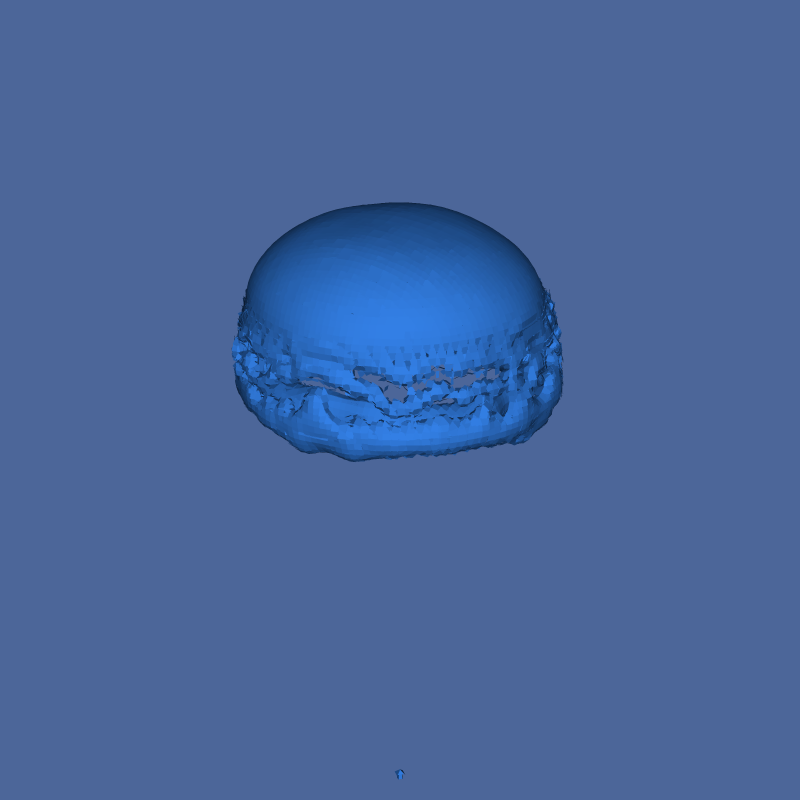
\includegraphics[width=\textwidth]{bulle3d_rupture.png}\\
      {\scriptsize Interface sous-resolue (ancien maillage).}
    \end{column}
  \end{columns}
  \vspace{0.4em}
  \begin{center}
    \footnotesize \textcolor{warnred}{\textbf{Avertissement :}} ces figures
    proviennent de l'\textbf{ancien code} (maillage defaillant). Elles illustrent
    la phenomenologie ; les valeurs quantitatives seront \emph{toutes} reprises
    avec le code precis.
  \end{center}
\end{frame}

%==============================================================================
\section{Suite du stage}
%==============================================================================
\begin{frame}{Semaine 5 et au-dela}
  \begin{columns}[T]
    \begin{column}{0.5\textwidth}
      \textbf{Cloture de la partie 1}
      \begin{itemize}
        \item Finir le precurseur lvl 9 stationnaire.
        \item Caracterisation THI propre (la \emph{bonne} version).
        \item Etude de convergence 7/8/9 \emph{reelle} (maillages enfin
              distincts) $\to$ vitesse terminale convergee.
      \end{itemize}
    \end{column}
    \begin{column}{0.5\textwidth}
      \textbf{Etude principale (objectif du stage)}
      \begin{block}{Intensite turbulente $\to$ vitesse d'ascension}
        \footnotesize
        A $Bo=1$ et $R_0$ fixes, faire varier l'intensite du forcage
        ($u_{rms}$) et mesurer :
        \begin{itemize}
          \item la vitesse d'ascension terminale $u_z$,
          \item le coefficient de trainee
                $C_D = \dfrac{4\,g\,d_{eq}\,(\rho_1-\rho_2)}{3\,\rho_1\,u_z^2}$,
          \item la deformation ($\chi$, aire interfaciale).
        \end{itemize}
      \end{block}
    \end{column}
  \end{columns}
  \vspace{0.3em}
  \begin{center}
    \footnotesize\itshape
    Vu le temps de calcul, on enchaine directement sur cette etude d'intensite
    des que la partie 1 est bouclee.
  \end{center}
\end{frame}

\begin{frame}{Synthese}
  \begin{columns}[T]
    \begin{column}{0.5\textwidth}
      \textbf{Acquis}
      \begin{itemize}
        \item Chaine DNS 3D Basilisk operationnelle (precurseur $\to$ bulle).
        \item Protocole d'injection en THI stationnaire.
        \item Diagnostics bulle complets (trajectoire, $u_z$, $\chi$, fragments).
        \item Maitrise de l'usage HPC (Kairos / CALMIP).
      \end{itemize}
    \end{column}
    \begin{column}{0.5\textwidth}
      \textbf{Lecons \& points ouverts}
      \begin{itemize}
        \item Une adaptation de maillage mal calibree peut \emph{invalider
              silencieusement} toute une etude de convergence.
        \item Resultats actuels = \textcolor{warnred}{ancien code}, a remplacer.
        \item A venir : caracterisation THI lvl 9 + influence de l'intensite
              turbulente sur l'ascension.
      \end{itemize}
    \end{column}
  \end{columns}
\end{frame}

%==============================================================================
\section{References et credits}
%==============================================================================
\begin{frame}{References et credits}
  \footnotesize
  \begin{block}{Code de reference}
    Implementation inspiree de la sandbox de \textbf{Wouter Mostert} :\\
    \texttt{https://basilisk.fr/sandbox/wmostert/turbulent\_bubble.c}\\
    (configuration precurseur THI + injection de bulle, advection VOF conservant
    la quantite de mouvement).
  \end{block}
  \begin{block}{Articles (J.~Fluid Mech., Cambridge University Press, 2021)}
    \begin{itemize}
      \item A.~Riviere, W.~Mostert, S.~Perrard, L.~Deike,
            \emph{Sub-Hinze scale bubble production in turbulent bubble
            break-up} (29 avril 2021).
      \item S.~Perrard, A.~Riviere, W.~Mostert, L.~Deike,
            \emph{Bubble deformation by a turbulent flow} (9 juin 2021).
    \end{itemize}
  \end{block}
  \begin{block}{Cadre}
    Stage IMFT --- ENSEEIHT / Toulouse INP. Tuteurs : D.~Legendre \& R.~Zamansky.
    Solveur \textbf{Basilisk} (S.~Popinet et coll.). Calculs : Kairos (IMFT),
    CALMIP / Olympe (projet P0910).
  \end{block}
\end{frame}

{\setbeamertemplate{footline}{}
\begin{frame}[plain]
  \centering
  \vfill
  {\Large\bfseries\color{imftblue} Merci de votre attention}\\[0.4cm]
  {\normalsize Questions \& discussion}\\[0.8cm]
  
\includegraphics[height=1.0cm]{logo_enseeiht.png}\hspace{1.2cm}
  
\includegraphics[height=1.0cm]{logo_imft.png}
  \vfill
\end{frame}}

\end{document}
